\chapter{Considerações Finais}
\label{c.conclusao}

Devido ao número de voluntários que participaram do estudo, não é possível generalizar os resultados obtidos. No entanto, as análises realizadas mostram uma tendência de preferência dos usuários. 

De acordo com a análise ANOVA realizada, a variância das avaliações não mostrou diferença significativa. Com esta informação, pode-se concluir que, para aplicações que envolvem poucas entradas de dados, os controles apresentados conseguem propiciar usabilidade satisfatória aos usuários. Na aplicação desenvolvida, o usuário pôde contar com três opções de entrada: clicar em um objeto selecionado, agachar e retornar ao menu principal. No caso do Google Cardboard 2.0, a última ação (retornar ao menu principal) não pôde ser efetuada através do controle, por isso, a aplicação contou com um botão virtual no ambiente, o que gerou alguns comentários negativos devido a necessidade do usuário de se locomover até o botão. 

O desenvolvimento deste projeto demonstrou que, se é intenção do usuário utilizar o Google Cardboard 2.0 como forma de entrada, é necessário preparar o ambiente adicionando elementos guias e botões adicionais, o que não seria necessário para os outros controles que possuem um número de botões elevado. Além disso, o usuário possui maior flexibilidade para se locomover no ambiente por meio dos botões direcionais físicos do controle do que através dos objetos guias no ambiente virtual (que limitam o número de posições dentro do cenário). Ao adicionar estes objetos, os botões direcionais dos controles tiveram sua utilidade anulada, deixando grande parte das opções de entrada de dados destes dispositivos inutilizada.

A partir destas informações, é recomendável que o desenvolvedor escolha um controle principal de acordo com as características da aplicação a ser desenvolvida. Para aplicações que envolvem somente a movimentação da cabeça e o clique para seleção, o Google Cardboard 2.0 é o controle mais apropriado, pois mostrou ser intuitivo e de fácil configuração. Aplicativos como \textit{VR Roller Coaster}, Netflix VR e Sistema solar VR disponíveis na Google Play \cite{googleplay}, são exemplos de aplicações desenvolvidas visando principalmente a utilização do Google Cardboard.

Já o teclado, apesar dos usuários terem experiência com este dispositivo, foi considerado o controle menos apropriado para aplicações em RV. Isto deveu-se principalmente pela quantidade excessiva de botões e pelo tamanho do dispositivo que trouxe certo desconforto aos usuários. O número de botões não interfere na usabilidade quando a quantidade de ações é pequena pois, por já possuírem experiência com o dispositivo, os usuários não apresentaram problemas para lembrar a localização de três botões. No entanto, ao aumentar o número de ações, botões no teclado podem ser facilmente confundidos e, como aplicações em RV não permitem que o usuário olhe para o controle a fim de encontrar o botão apropriado, seria necessário sair da experiência removendo o capacete de visualização. Quanto ao tamanho, comentários e observações feitos durante a análise demonstraram que o teclado foi o controle mais desconfortável comparado aos outros dispositivos apresentados. Uma característica positiva do teclado no entanto, é a conexão sem fio, que garante maior liberdade de movimentação. 

Os controles que garantiram maior satisfação dos usuários no quesito usabilidade foram os controles PS2 e VR Box. Estes últimos são conhecidos por serem utilizados em jogos e apresentam um número de botões satisfatório. Durante a análise, todos os usuários demonstraram ter experiência com o controle do PS2 e não apresentaram dificuldade para encontrar os botões corretos no dispositivo. Apesar de apenas um participante ter declarado possuir experiência com o VR Box, nenhum dos usuários apresentou problemas para encontrar os botões corretos. No entanto, houve comentários negativos como a distância entre os botões ser muito próxima e botões no centro do controle serem facilmente confundidos, o que seria um problema caso estes botões resultassem em ações diferentes (na aplicação apenas um botão do centro resultava em uma ação).

A grande diferença entre os controles preferidos, no entanto, foi a conexão com o \textit{smartphone}. Enquanto o VR Box é conectado ao celular através do \textit{Bluetooh}, o PS2 utilizou o cabo do próprio dispositivo, um adaptador e um cabo OTG para realizar a conexão, além de ser necessário um aplicativo para reconhecer o controle como um dispositivo de entrada devido a versão do Android utilizada. Apesar desta dificuldade, existem controles semelhantes à este que apresentam formas de conexão sem fio, como o controle do console XBOX (Figura ~\ref{f.xbox}) que realiza conexão Wifi e do console Playstation 4 (DUALSHOCK®4) que utiliza o \textit{Bluetooth} para se conectar com o dispositivo e pode ser visualizado na Figura ~\ref{f.ps4}.

\begin{figure}[H]
	
	\begin{minipage}{.5\textwidth}{
			\centering
			\captionof{figure}{\small Controle XBOX}
			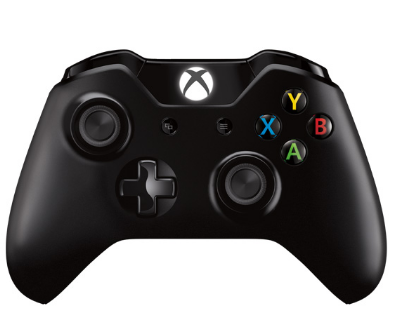
\includegraphics[height=5cm]{Imagens/xbox.png}		
			\label{f.xbox}
			\legend{\small Fonte: \citeonline{xbox}}	
		}
	\end{minipage}
	\begin{minipage}{.5\textwidth}{
			\centering
			\captionof{figure}{\small DUALSHOCK®4}
			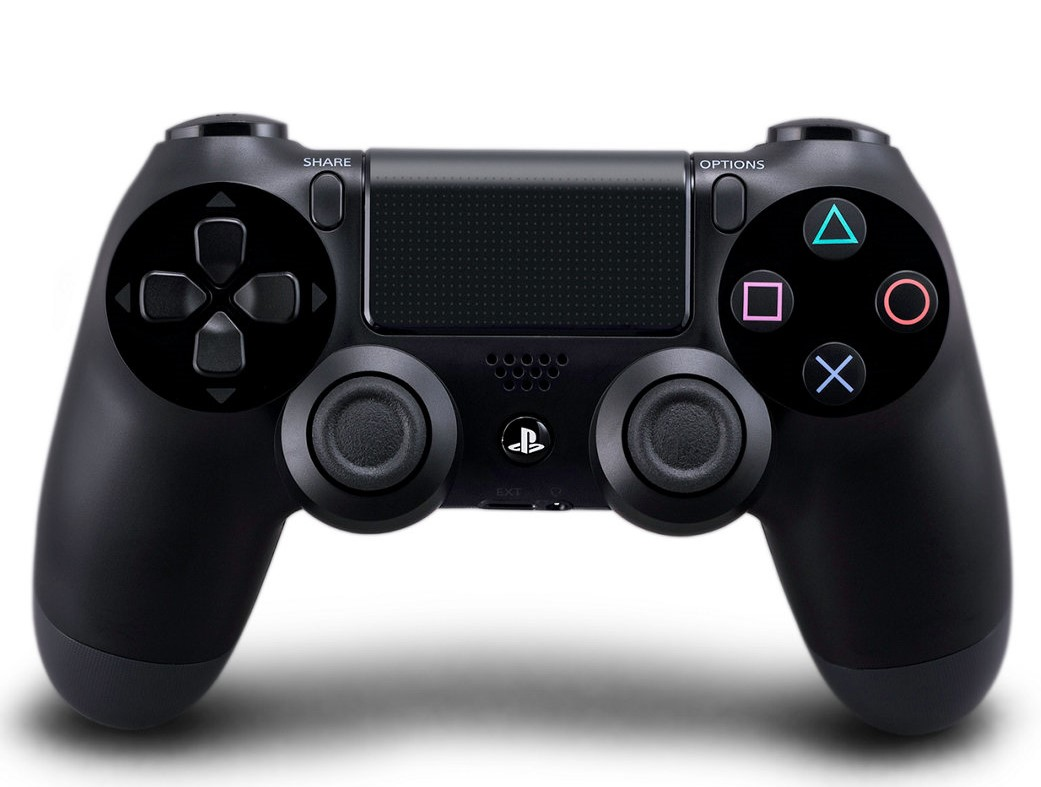
\includegraphics[height=5cm]{Imagens/dualshock4.jpg}		
			\label{f.ps4}	
			\legend{\small Fonte: \citeonline{ps4}}
		}
	\end{minipage}
\end{figure}


A utilidade destes controles no ambiente virtual pode ser reforçada devido ao fato de a empresa Oculus® oferecer o controle do XBOX juntamente com o seu óculos de realidade virtual (Rift). \cite{oculushome} 

A vantagem do VR Box em comparação com o PS2, PS4 e XBOX é a liberdade de movimentação do usuário pois o primeiro exige somente uma das mãos para se obter a experiência completa enquanto os últimos necessitam que o controle seja manejado com as duas mãos. Com a flexibilidade do VR Box, é possível adicionar sensores de movimentação no controle que captam a localização dos braços do usuário, possibilitando a criação de aplicações ainda mais imersivas, alterando a tecnologia para Virtualidade Aumentada. A empresa Oculus® além do controle XBOX, também oferece ao usuário a possibilidade de adquirir um segundo controle denominado Oculus Touch (Figura ~\ref{f.oculustouch}). Este apresenta a flexibilidade oferecida pelo VR Box e utiliza os sensores de movimento para o mapeamento dos braços do usuário na aplicação. 

\begin{figure}[H]
	\caption{\small Oculus Touch}
	\centering
	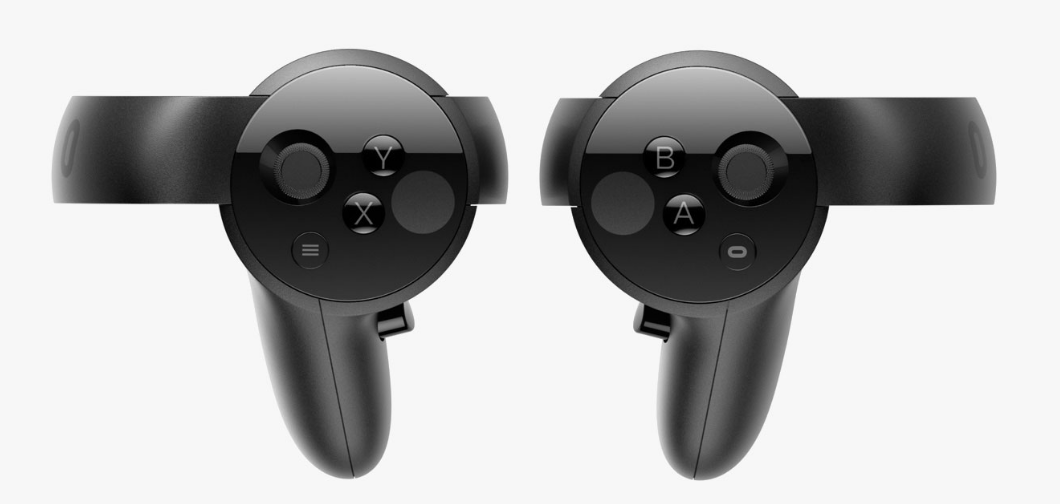
\includegraphics[height= 5cm]{Imagens/oculustouch.png}
	\label{f.oculustouch}
	\legend{\small Fonte: \citeonline{oculushome}}
\end{figure}

Estudos recentes demonstraram que é possível criar um controle como o Oculus Touch com um preço acessível. Os pesquisadores Fangwei Lee e Shuo Zhang desenvolveram o projeto RealTrigger \cite{realtrigger}. O projeto consiste em um controle feito a partir de papelão onde um \textit{QR code} é posicionado no mesmo de forma que a aplicação reconheça o código e mapeie este para a aplicação. O controle pode ser visualizado na Figura ~\ref{f.realtrigger}. 

\begin{figure}[H]
	\caption{\small RealTrigger}
	\centering
	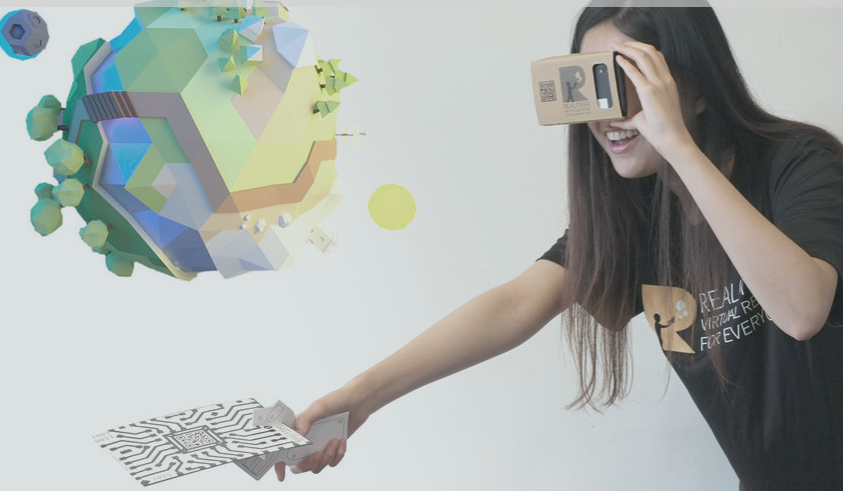
\includegraphics[height= 7cm]{Imagens/realtrigger.png}
	\label{f.realtrigger}
	\legend{\small Fonte: \citeonline{realtrigger}}
\end{figure}

\begin{citacao}
	"Nós pensamos que experiências imersivas deveriam ser acessíveis para qualquer pessoa independente da situação econômica e foi por isso que desenvolvemos o RealTrigger: O controle de RV mais acessível que pode proporcionar uma experiência completa de interação em RV." \cite[tradução nossa]{realiteer}
\end{citacao}

Utilizar o RealTrigger juntamente com o VR Box ou outro \textit{joystick} poderia oferecer um controle imersivo acessível e com uma quantidade de ações e liberdade de movimento satisfatórias. 

De modo geral, a escolha do controle irá depender dos objetivos da aplicação. Aplicações que requerem muitas ações distintas do usuário devem contar com um controle externo como o VR Box ou controles utilizados em vídeo games como o PS4 e o XBOX. Controles que possuem conexão Wifi ou \textit{Bluetooth} são preferíveis por garantirem maior conforto e facilidade de conexão. Já aplicações que exigem apenas uma ação do usuário (normalmente o clique), podem contar com um controle mais simples como o Google Cardboard. 







